\section{Introduction}\label{introduction}

Are democratic commitment and nationalism opposed? They are widely assumed to be, because democratic ideals of equality and inclusion appear difficult to reconcile with nationalist claims that distinguish insiders from outsiders. So citizens who prize the first should resist the second. The assumption organizes a large empirical literature. Studies of European publics report that an ethnic conception of nationhood depresses support for democracy \citep{gabrielsson2025} and predicts hostility to immigrants \citep{hjerm1998, pehrson2009}, and recent comparative work often treats the negative relationship as near-universal. The same premise frames the literature on Chinese popular nationalism. \citet[p.~62]{zhong2020} note that ``people with more liberal democratic values tend to be less nationalistic'' before reporting the opposite for China, as does later nationwide work \citep{liu2026}.

Yet this assumption that democratic commitment and nationalism are inherently opposed outruns the evidence and rests on a simplified reading of both concepts. The two developed together in the modern era, and liberal-nationalist theorists have long argued that national solidarity can sustain democratic self-government rather than undermine it \citep{tamir2019}. Recent work presses the point with new evidence. Hur \citeyearpar{hur2022narratives, hur2026democratic} shows that national attachment has underwritten democratic civic duty in South Korea, so that nationalism can strengthen democracy rather than corrode it. I share that starting point but reach it by disaggregating each concept, which brings a complication into view that a duty-centered account leaves aside. Where nationhood is ethnically bounded, as in Korea, commitment to democratic rights ceases to restrain the exclusionary face of nationalism. More fundamentally, neither ``democracy'' nor ``nationalism'' is a single attitude. Each is a bundle of distinct orientations, and how they relate depends on which components one has in mind and in which countries and regions one examines them.

This is an especially useful moment to revisit the question. Nationalism has returned to the center of political debate, where it is frequently equated with nativism, democratic backsliding, and right-wing populism \citep{mudde2007, brubaker2017}. At the same time, new comparative data make it possible to test a long-standing assumption that has more often been asserted than examined, and to do so beyond the Western democracies on which the prevailing verdict was largely built. The 2023 ISSP National Identity and Citizenship module is the only cross-national survey that measures the content of nationhood and multiple forms of nationalism alongside citizens' democratic commitments. Fielded in 29 countries, including consolidated Western democracies, post-communist Europe, several electoral autocracies, the institutionally liberal democracies of East Asia, and others such as Israel, Mexico, and South Africa, it opens an opportunity to examine when democratic commitment and nationalism coincide and when they conflict.

This article therefore disaggregates both concepts and asks a more precise question: for which components, and under what conditions, is commitment to democracy antagonistic to nationalism? There are two main findings to report. 

First, democratic commitment and nationalism are not general opposites. Endorsement of liberal-democratic rights is essentially unrelated to ordinary national pride, while perceived democratic performance is positively associated with pride and even with national superiority across regions. Democratic commitment opposes the narrower exclusionary face of nationalism, above all hostility toward immigrants. Second, even this conflict is conditional. The negative association between democratic-rights endorsement and exclusion is strongest where the nation is imagined in civic terms and weakens, disappears, or even reverses where membership is understood in ethnocultural terms.

This conditional pattern matters theoretically because it is not what a focus on regime type would predict. The pattern is governed by the civic-versus-ethnic content of nationhood rather than by the liberal-democratic quality of political institutions. South Korea and Taiwan, for example, have converged on the institutions of liberal democracy, yet citizens who value democratic rights are no less exclusionary and are somewhat more attached to ascriptive conceptions of nationhood. In multilevel models, the content of nationhood moderates how strongly democratic-rights endorsement restrains exclusion, while institutional liberalism (V-Dem's liberal component) adds no detectable moderation of its own once the content of nationhood is included.

The contribution of this article is to revise a stubborn assumption. Democratic commitment and nationalism do not stand in a generally antagonistic relationship. The conflict is confined to liberal-democratic rights and the exclusionary face of nationalism, and only where nationhood is understood in civic terms. Following Tamir \citeyearpar{tamir2019}, the relevant divide is often between liberal and illiberal orientations rather than between democracy and nationalism as such. And following the contextual logic of Pehrson, Vignoles, and Brown \citeyearpar{pehrson2009}, whether that divide becomes politically meaningful depends on how the national community is bounded. I show that the same contextual logic governs the relationship between democratic commitment and exclusion, and I pit the content of nationhood directly against institutional liberalism. The apparent law that democracy restrains nationalism turns out to be a feature of civic-national political cultures rather than a property of democratic commitment itself. This matters when nationalism is routinely equated with nativism and right-wing populism, because it shows what restrains exclusion and in which countries.

\section{Disaggregating democracy and nationalism}\label{disaggregating-democracy-and-nationalism}

Neither key term denotes a single attitude. Treating democracy and nationalism as bundles of distinct orientations helps explain the conflicting findings in the literature.

Regarding democracy, two orientations must be kept apart. The first is normative commitment to the \emph{principles} of liberal democracy, especially the rights that protect minorities and enable participation and dissent. The second is evaluation of democratic \emph{performance}, how well the system is seen to work. Norris \citeyearpar{norris1999} documented that publics distinguish principled support from performance satisfaction, and that the two need not coincide. The distinction matters because ``democracy'' is a contested concept. People endorse it while loading it with majoritarian or authoritarian meaning, and abstract support conceals ``illiberal democrats'' who reject the liberal principles that define the regime \citep{kirsch2019, schedler2007}. The ISSP allows the separation directly, asking how important various rights are \emph{for democracy} (principles) and, separately, how well democracy \emph{works today} (performance).

For nationalism, the relevant distinction is between \emph{exclusionary} content and ordinary \emph{attachment}. Since Kosterman and Feshbach \citeyearpar{kosterman1989}, survey research has separated chauvinism and perceived superiority from patriotic pride, and recent work treats popular nationalism as a set of separable components rather than a single thing \citep{bonikowski2016asr, bonikowski2017}. The exclusionary components include an ascriptive definition of who truly belongs (by birth or ancestry), beliefs in national superiority, and hostility to immigrants, central to nativism \citep{mudde2007}. National pride in collective achievements is conceptually distinct, and pride and exclusion need not co-occur \citep{hjerm1998}. Conflating them makes ``nationalism'' appear uniformly anti-democratic.

Putting the two disaggregations together yields the article's first expectation. If the tension is between liberal commitment and exclusion rather than between democracy and nationalism as such, democratic-rights endorsement should be negatively related to exclusionary nationalism and largely unrelated to national pride, while performance evaluations, which capture satisfaction rather than liberal principle, should relate positively to pride.

\begin{quote}
\textbf{E1 (two faces of nationalism).} Endorsement of liberal-democratic rights is negatively associated with exclusionary nationalism and essentially unrelated to national pride. Perceived democratic performance is positively associated with pride.
\end{quote}

The harder question is whether the negative rights--exclusion relationship holds everywhere. Two readings diverge here. On a regime-centered reading, \emph{institutional} liberalism is what restrains exclusion, so the negative relationship should strengthen with the liberal quality of a country's democracy. On a culture-centered reading, the \emph{content} of nationhood is what matters, so the relationship should depend on whether the nation is defined in civic or ethnic terms. Brubaker \citeyearpar{brubaker1992} distinguishes civic from ethnic traditions of nationhood.\footnote{The civic/ethnic distinction is a heuristic, not a strict binary or a typology of good and bad nationalisms, and a civic conception is not thereby fully inclusive \citep{simonsen2020civic}. The contrast lies in the kind of demand a community places on its members. Civic demands, such as participation and accepting shared institutions, are in principle achievable rather than ascribed at birth.} Using earlier ISSP rounds, Pehrson and colleagues \citeyearpar{pehrson2009} show that the link between national identification and anti-immigrant prejudice is conditional on the \emph{national definition} prevailing in a country. It is strong where nationhood is defined in ethnocultural (chiefly linguistic) terms and weak where it is defined civically. The two readings diverge for cases where they come apart, in particular East Asian democracies, institutionally liberal yet retaining strongly ethnic conceptions of the nation \citep{shin2006}.

\begin{quote}
\textbf{E2 (scope condition).} The negative association between democratic-rights endorsement and exclusion is moderated by the civic-versus-ethnic content of nationhood, not by institutional liberalism. It is strong where the prevailing conception is civic and weak or reversed where it is ethnic.
\end{quote}

E2 predicts cross-national heterogeneity in the rights--exclusion relationship, and it predicts that the heterogeneity tracks the content of nationhood rather than regime type.

\section{Data, measures, and approach}\label{data-measures-and-approach}

The data used here are the ISSP 2023 National Identity and Citizenship module \citep{issp2023}, 43,517 respondents in 29 countries. All items are rescaled to the unit interval, oriented so higher values mean more of the named concept. Descriptive estimates use the combined ISSP weight. The \emph{democratic-rights} measure averages three items on the importance for democracy of protecting minority rights, expanding participation, and permitting civil disobedience. \emph{Democratic performance} is the single item on how well democracy works today (SI-A gives full wording). Nationalism is split into ascriptive membership, civic membership, national superiority, anti-immigrant exclusion, protectionism, and national pride (excluding pride in democracy). Anti-immigrant exclusion is the primary outcome; ascriptive membership, superiority, and pride are secondary, and protectionism is set aside as conceptually distinct from exclusion. Individual controls are age, gender, education, and left--right self-placement. Country-level institutional liberalism comes from the Varieties of Democracy (V-Dem) project's liberal-component index (\texttt{v2x\_liberal}) for 2023, and its electoral component (\texttt{v2x\_polyarchy}) is the contrast \citep{vdem2025}. The SI gives full item wording, coding, and descriptive statistics (SI-A), with scale reliabilities in SI-C.

Two measurement issues deserve attention. The democratic-rights battery is unique to the 2023 module, so the central relationship cannot be traced over time, and the relational analysis is cross-sectional by necessity; the SI places the 2023 \emph{levels} of exclusionary nationalism in their 1995--2023 trajectory (SI-K). The attitude scales are also not fully comparable across these societies. Multi-group confirmatory factor analyses reproduce the expected factor structure (configural invariance holds) but decisively reject the equality of intercepts needed to compare scale \emph{means} (scalar invariance fails, with the comparative fit index dropping by 0.11 to 0.23). The loadings that govern \emph{associations} are more comparable, though the change in them modestly exceeds the conventional 0.01 threshold. I therefore treat metric invariance as approximate and compare within-context associations, not levels (SI-D). The anti-immigrant scale is the least equivalent of the set, so its country-level estimates are read with corresponding caution. This is the pattern earlier work documents for ISSP nationalism scales \citep{reeskens2010}.

Respondents are nested in countries, and I ask whether a within-person relationship varies across contexts. I therefore estimate multilevel models with random intercepts and a random slope on the democratic-rights index, centered on each country's mean so the slope is the within-country relationship. I then test whether that slope differs by two country-level features, the content of nationhood (the country mean of ascriptive membership, standardized across countries) and institutional liberalism (the standardized V-Dem liberal component), entered together so the two compete. I report unweighted model-based estimates in the main text and design-based weighted estimates as a robustness check in the SI, and they agree. The adjusted models are estimated on complete cases ($n = 37{,}177$ for anti-immigrant exclusion), limited mainly by missing left--right placement. Given the very large sample, I emphasize the size and sign of the within-country relationships rather than statistical significance. The cross-level interactions, by contrast, are identified from only 29 countries, so I corroborate them with a country-level second stage (SI-F) and read the institutional-liberalism comparison with corresponding caution.

\section{Results}\label{results}

\subsection{The conventional pattern is not universal}\label{the-conventional-pattern-is-not-universal}

The simple correlations already show that democratic-rights endorsement restrains exclusion only in the West. Within Western democracies, democratic-rights endorsement is negatively correlated with every exclusionary measure (−0.23 with anti-immigrant exclusion, −0.15 with ascriptive membership, −0.14 with superiority) and essentially zero with pride (−0.03). Outside the West the pattern frays and inverts. In the East Asian democracies the same endorsement is \emph{positively} correlated with ascriptive membership (+0.09), superiority (+0.07), and pride (+0.09), and unrelated to anti-immigrant exclusion (−0.02), and in the electoral autocracies the exclusionary correlations are positive. The full grid is in SI-H.

\subsection{The relationship reverses across countries}\label{the-relationship-reverses-across-countries}

Multilevel models confirm that the rights--exclusion relationship is not one fixed number but varies across countries. Across the four outcomes the random slope has a standard deviation between 0.10 and 0.14, as large as or larger than the average slope itself, so how much the relationship differs across countries matters as much as its average. Conceptions of nationhood are themselves highly clustered by country (intraclass correlation 0.32 for ascriptive membership). Figure 1 plots the country-specific adjusted slopes for anti-immigrant exclusion. They range from about −0.33 in the United States to +0.30 in Hungary, with Western democracies at the negative end and the two East Asian democracies at zero (SI-I gives the other outcomes).

\begin{figure}[ht]
\centering
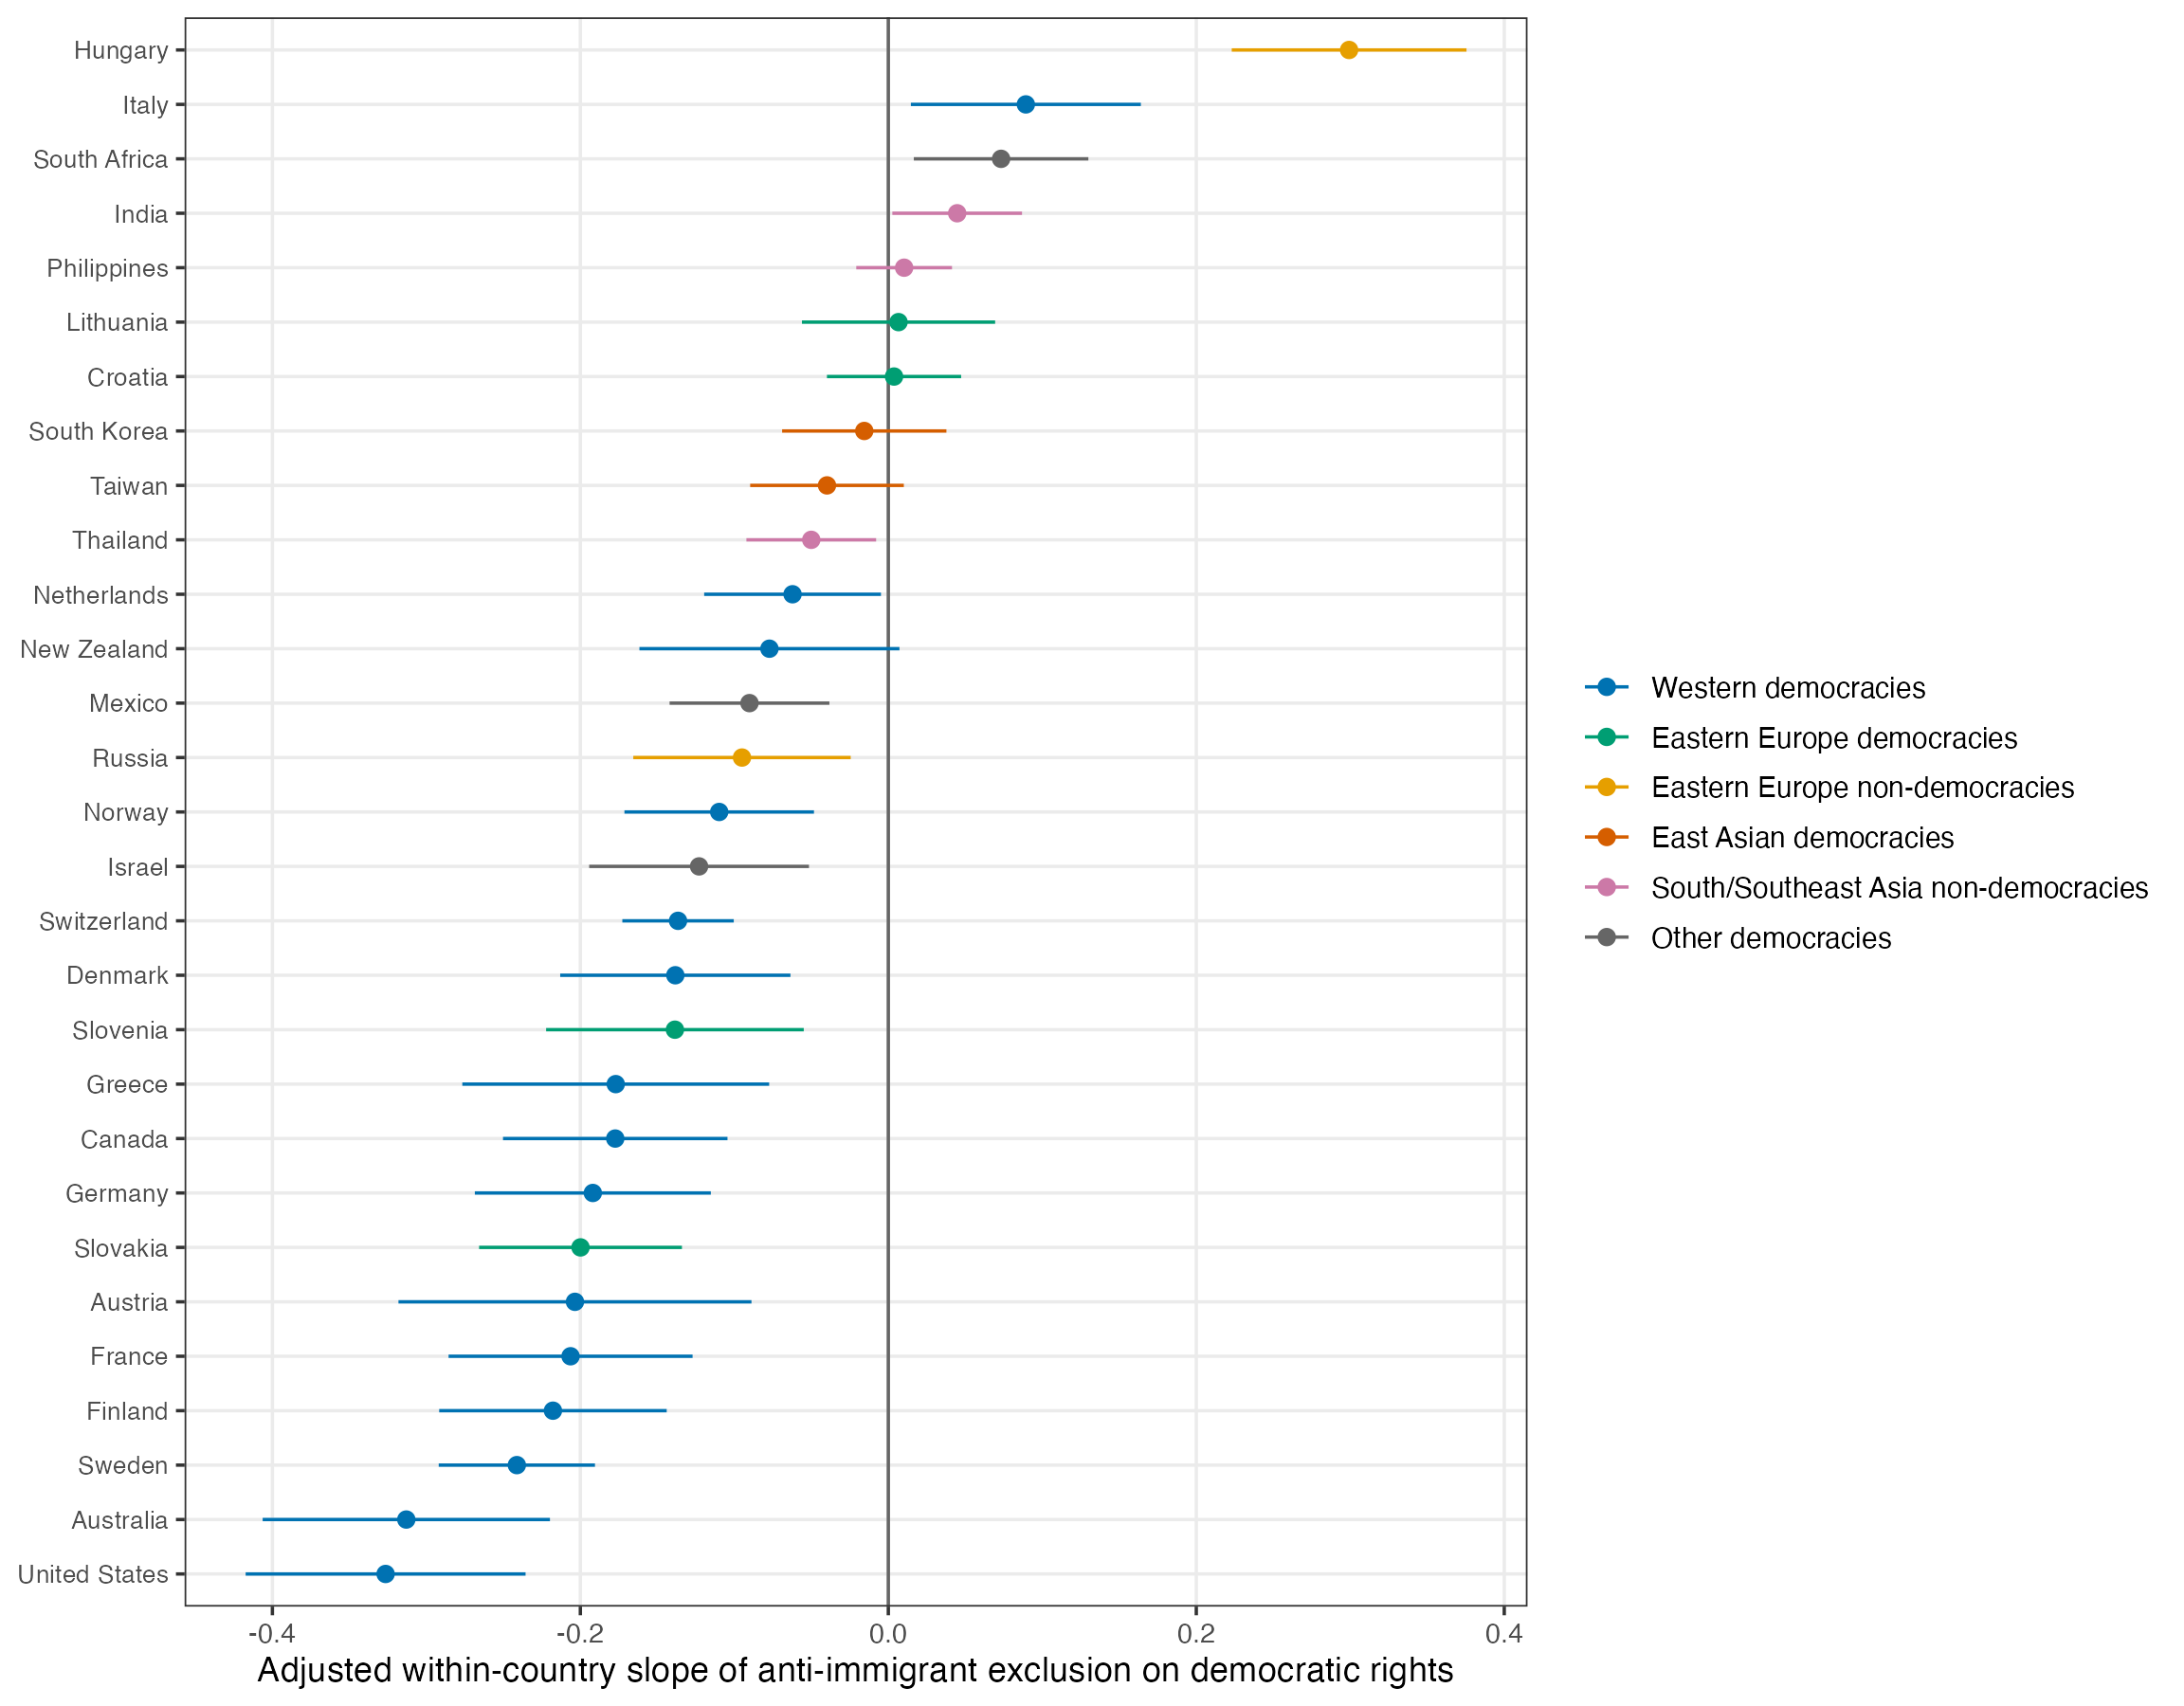
\includegraphics[width=0.66\linewidth,height=\textheight,keepaspectratio,alt={Cross-national heterogeneity in the relationship between democratic-rights endorsement and anti-immigrant exclusion. Points are country-specific adjusted within-country slopes, colored by region-regime group.}]{figures/fig2_random_slopes.png}
\figcap{Cross-national heterogeneity in the rights--exclusion relationship}{Each point is a country's \emph{within}-country slope of anti-immigrant exclusion on democratic-rights endorsement, adjusted for age, gender, education, and left--right placement; bars are 95\% confidence intervals. Color denotes region-regime group, and the vertical line marks zero, so negative values mean democratic-rights endorsement restrains exclusion. $n = 37{,}177$ complete cases in 29 countries.}
\end{figure}

\subsection{National content, not political institutions}\label{content-not-institutions}

What accounts for the spread? Figure 2 puts the two candidate moderators side by side. Where the nation is imagined in civic terms, as in Canada, the United States, and Sweden (the low-ascriptive end of Panel A), rights endorsement strongly restrains exclusion. Where it is imagined ethnically, the restraining relationship vanishes (Panel A, r = 0.65). Against institutional liberalism the slopes are weak and scattered (Panel B, r = −0.33), and South Korea and Taiwan score high on V-Dem's liberal component yet sit at the zero line, alongside far less liberal cases.

\begin{figure}[ht]
\centering
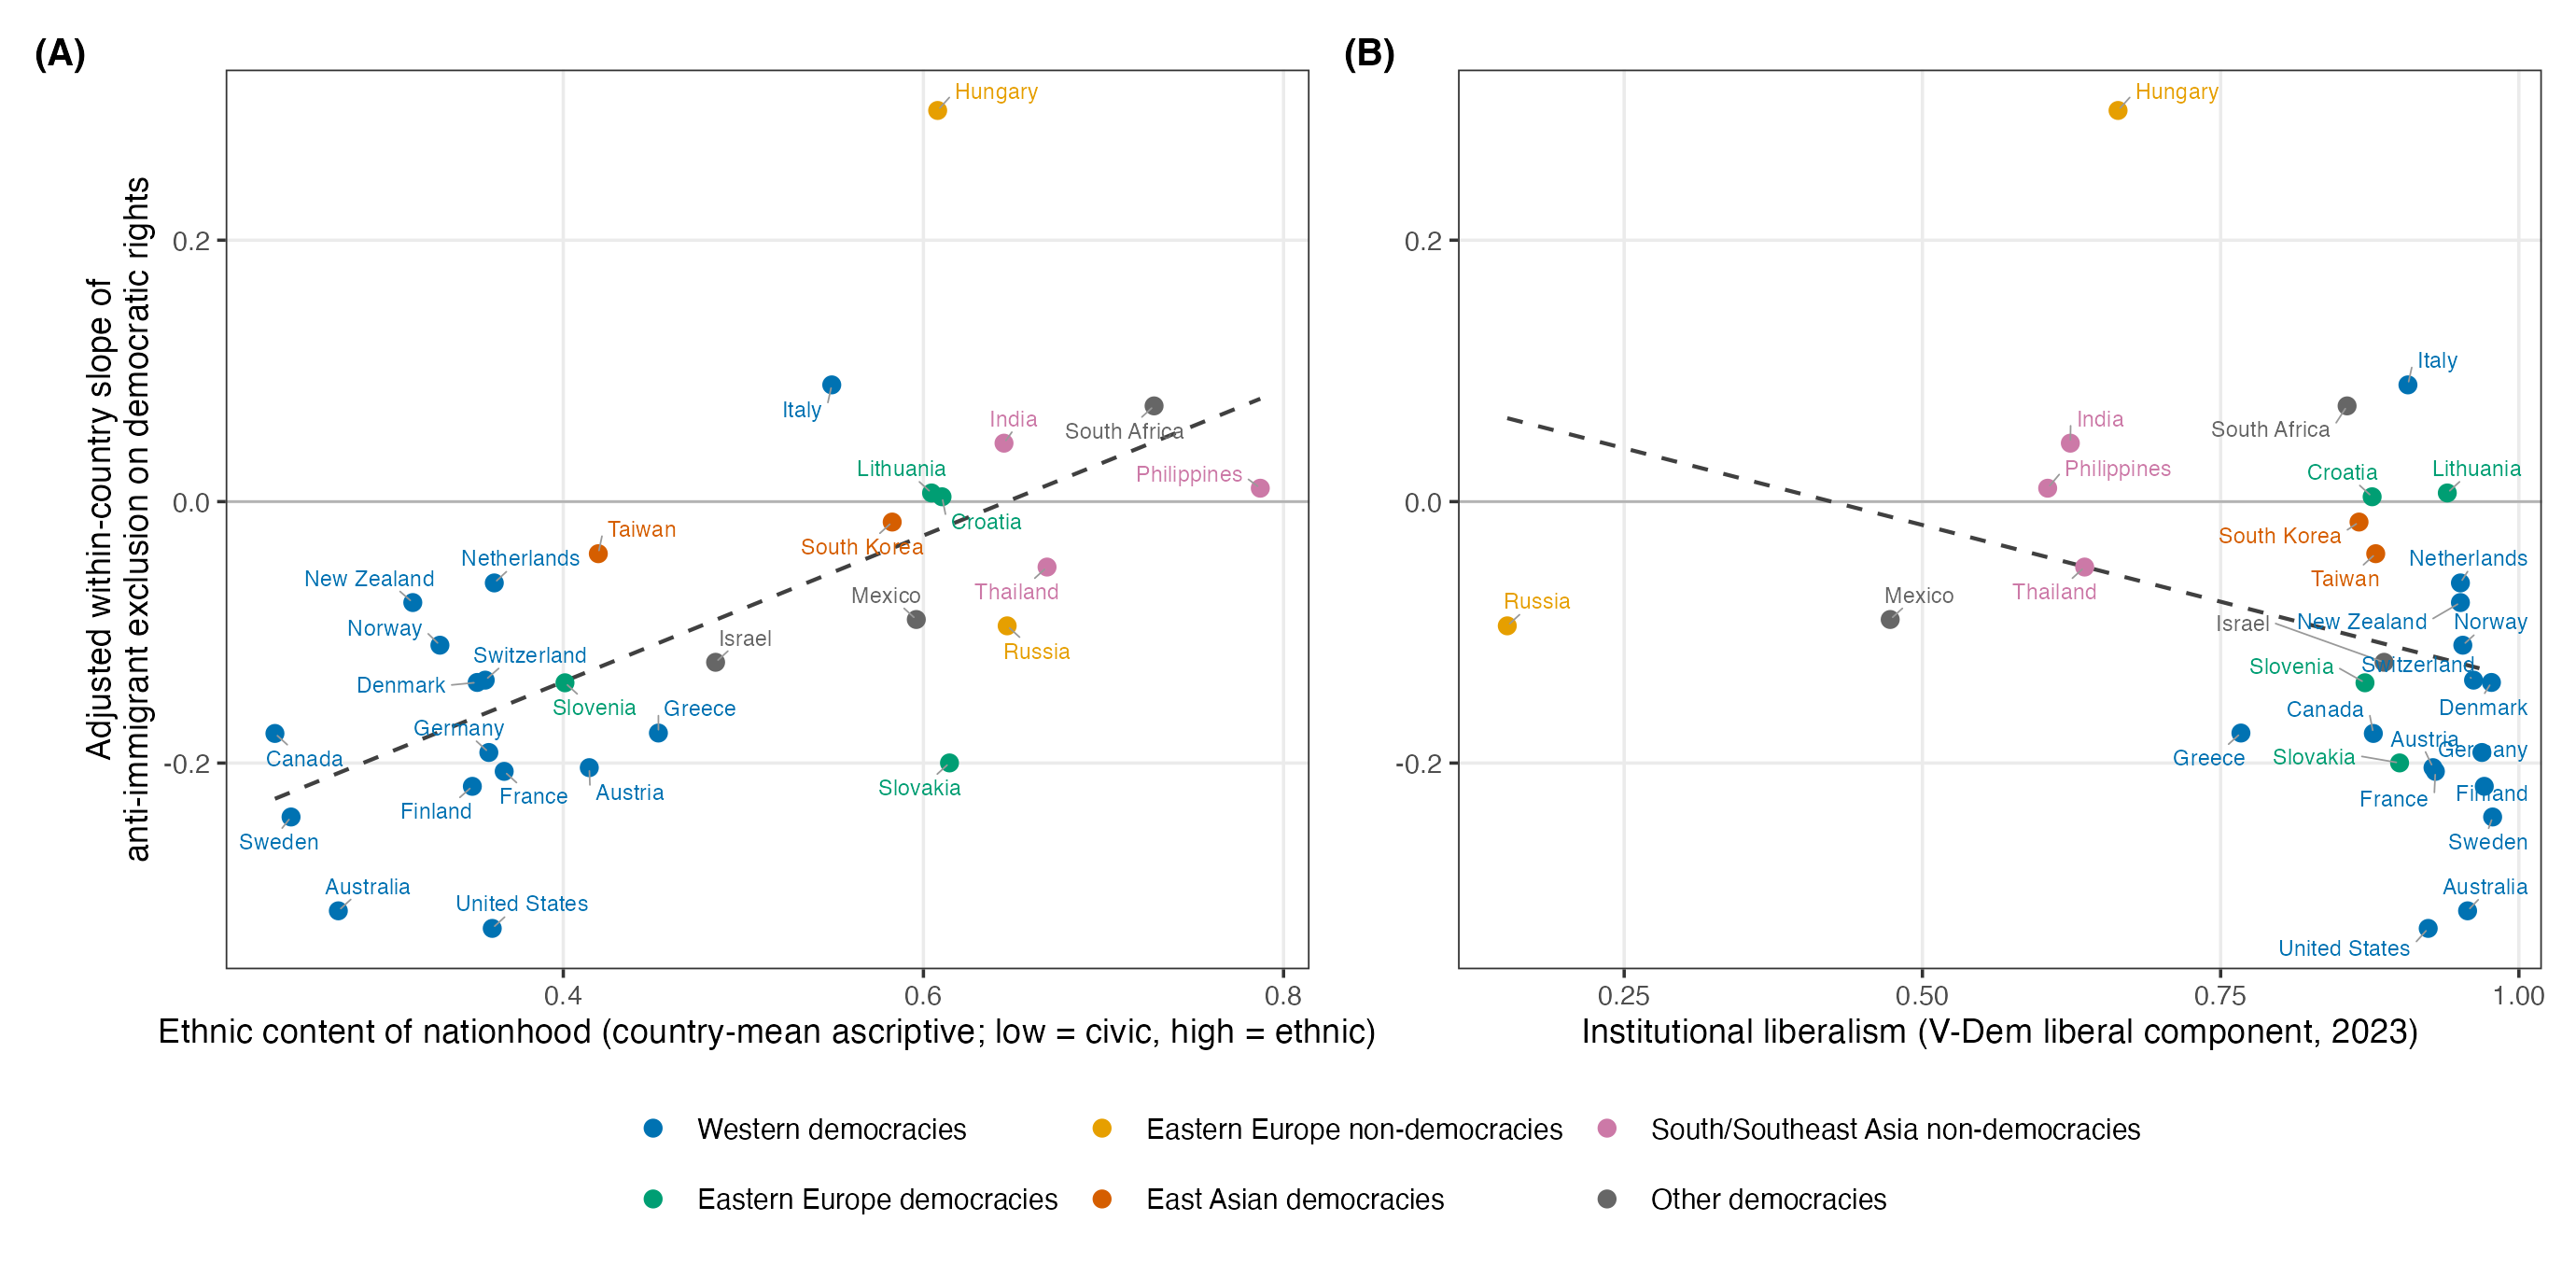
\includegraphics[width=0.72\linewidth,height=\textheight,keepaspectratio,alt={Country-specific adjusted slopes of anti-immigrant exclusion on democratic-rights endorsement, plotted against two candidate moderators. Panel (A) plots the civic--ethnic content of nationhood (country-mean ascriptive membership). Panel (B) plots institutional liberalism (V-Dem liberal component, 2023). Each point is a country, and the dashed line is the bivariate fit.}]{figures/fig1_moderation.png}
\figcap{The content of nationhood moderates the rights--exclusion slope; institutional liberalism does not}{Each point is a country, plotting its adjusted slope (as in Figure 1) against a candidate moderator; the dashed line is the bivariate fit. Panel (A) uses the civic--ethnic content of nationhood (country-mean ascriptive membership; low values civic, high ethnic), where the association is strong ($r = 0.65$). Panel (B) uses institutional liberalism (V-Dem liberal component, 2023), where it is weak and scattered ($r = -0.33$). South Korea and Taiwan score high on V-Dem's liberal component yet sit at the zero line.}
\end{figure}

The multilevel models settle the comparison by entering both moderators at once (full coefficients, random effects, and implied slopes in SI-E). The cross-level interaction between democratic-rights endorsement and the ethnic content of nationhood is positive and clearly estimated for anti-immigrant exclusion (b = 0.108, SE = 0.027) and for ascriptive membership (b = 0.088, SE = 0.027). The interaction with institutional liberalism, entered in the same model, is indistinguishable from zero (b = 0.020, SE = 0.027 for anti-immigrant exclusion, and b = −0.006 for ascriptive membership). Institutional liberalism shows no detectable independent moderation once the content of nationhood is in the model. A country-level second stage returns the same verdict (SI-F). In the content-only model, the implied within-country slope for anti-immigrant exclusion weakens from −0.22 where the nation is civic (one standard deviation below the mean on ethnic content) to −0.03 where it is ethnic (one standard deviation above). For ascriptive membership it crosses zero, from −0.13 to +0.05. The reversal is not an artifact of the regime classification, the choice of index, or the weighting scheme (Section SI-J).

\subsection{Two faces of democratic commitment}\label{two-faces-of-democratic-commitment}

The two democracy measures relate to nationalism in opposite ways, and that contrast shows where democracy and nationalism align. Figure 3 contrasts the pooled within-country slopes for democratic \emph{principles} (rights endorsement) and democratic \emph{performance} (full models in SI-G). Principled commitment is negative for the exclusionary outcomes and weakly positive for pride, at −0.12 for anti-immigrant exclusion, −0.05 for superiority, −0.04 for ascriptive membership, and +0.05 for pride. Democratic \emph{performance} runs in the opposite direction. People who think democracy works well are markedly \emph{prouder} of their country (0.26), more likely to endorse national \emph{superiority} (0.14), and more attached to civic membership (0.08), even as they too are less anti-immigrant (−0.14). This positive tie between democratic performance and pride, and even chauvinism, holds in every region, and it is the plainest sign that democratic commitment and nationalism are not opposed.

\begin{figure}[ht]
\centering
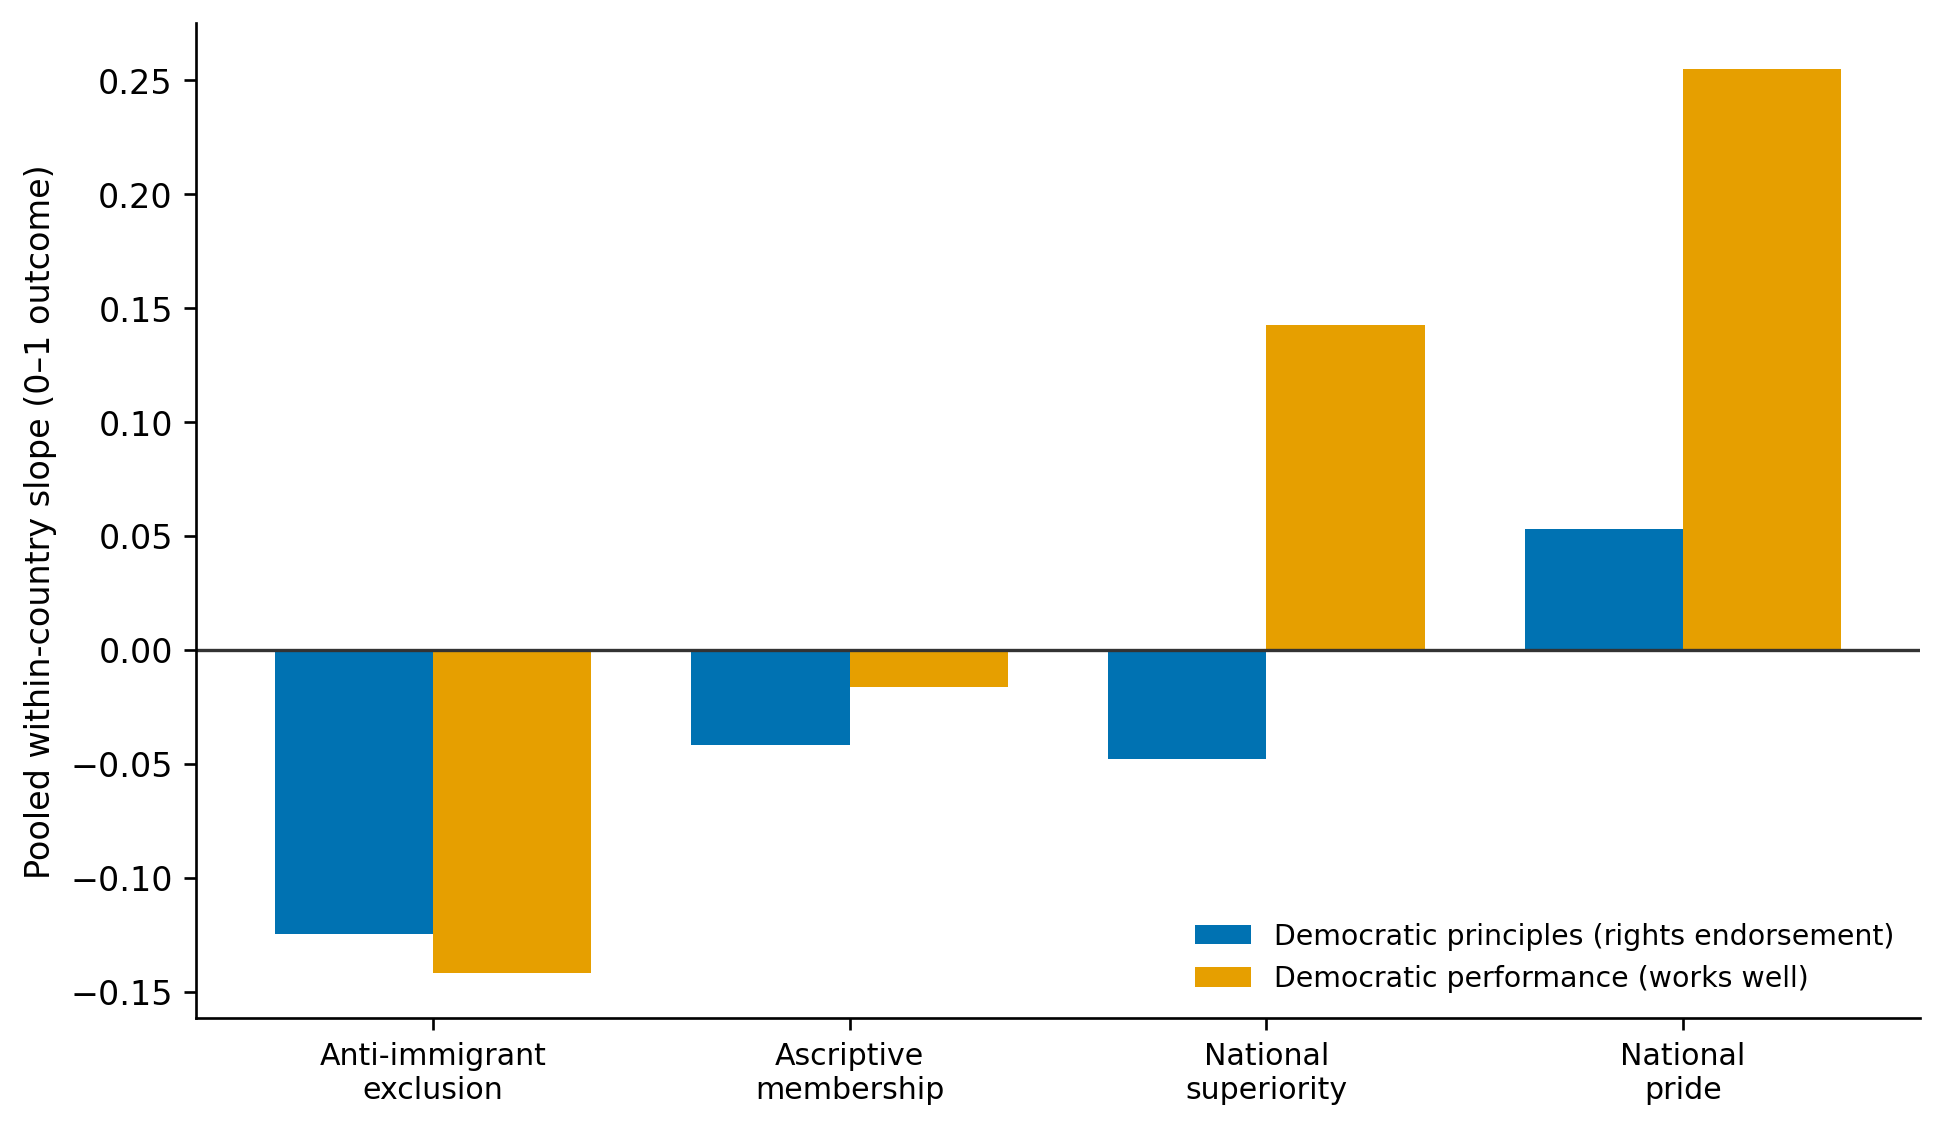
\includegraphics[width=0.62\linewidth,height=\textheight,keepaspectratio,alt={Two faces of democratic commitment. Pooled within-country slopes for democratic principles (rights endorsement) and democratic performance, by nationalism outcome. Principled commitment restrains exclusion without dampening pride, while performance travels with pride and superiority.}]{figures/fig3_two_faces.png}
\figcap{Two faces of democratic commitment}{Pooled within-country slopes of each nationalism outcome on two democracy measures, democratic principles (endorsement of liberal-democratic rights) and democratic performance (how well democracy is seen to work). Principled commitment restrains exclusion without dampening pride, whereas performance evaluations travel \emph{with} pride and superiority. Full performance models are in SI-G.}
\end{figure}

One performance result is mechanical. People who rate democracy as working well are, unsurprisingly, prouder of ``the way democracy works,'' a near-tautology sometimes reported as a finding. The substantive result is the positive association with pride in non-democratic achievements and with superiority.

\section{Discussion}\label{discussion}

The central finding is easy to misstate, so it is best to be precise. Democratic commitment and nationalism are not general opposites. National pride is untouched by liberal commitment and rises with satisfaction in democratic performance. Democratic commitment restrains only the exclusionary face of nationalism. Even that restraint depends on how the nation is imagined. It holds where the nation is imagined in civic terms and lapses where it is imagined ethnically, governed by the content of nationhood rather than the liberal quality of institutions. Tamir \citeyearpar{tamir2019} states this more clearly. The real divide runs between liberal and illiberal orientations, and whether it surfaces depends on how the nation draws its boundaries.

The East Asian democracies are especially instructive about regional difference, and they complicate readings centered on regime type. By V-Dem's measures and the broader scholarly consensus, Taiwan and South Korea have converged on the institutions of liberal democracy, yet their citizens who most value democratic rights are no less exclusionary and are somewhat more attached to an ascriptive nation.\footnote{Taiwan and South Korea differ. South Korea's genealogical conception of the nation remains strong \citep{hur2022narratives, jo2024nations}, whereas Taiwan has reoriented toward a civic, territorial self-understanding defined against the Han nationalism of the mainland and bound up with its democracy \citep{wachman1994taiwan, ho2022desinicizing}. A comparative list experiment across the two cases documents the contrast \citep{denney2026conformity}. Taiwan's mean ascriptive endorsement (0.42) falls below South Korea's (0.58), so the restraining relationship flattens rather than reverses there.} The likeliest reason is historical rather than institutional. In Korea and Taiwan, national mobilization was bound up with democratization \citep{shin2006, chu2004}, and a genealogical or ethnic understanding of the nation carried into the democratic era \citep{shin2006}. Where democracy was built by affirming the nation, democratic commitment and national attachment are complements, and ``democratic rights'' are understood inside a national project rather than against its ethnic boundaries. This complementarity is what Hur's \citeyearpar{hur2022narratives, hur2026democratic} account of Korea describes, in which national attachment supplies the civic duty that sustains democratic participation. The evidence presented here is consistent with that account and draws out its less benign corollary. The ethnically grounded nationhood that makes nationalism a democratic resource is what keeps democratic-rights commitment from restraining exclusion, so the restraint typical of the civic West is absent in Korea rather than merely weaker. This also reframes the ``puzzle'' of Chinese popular nationalism, in which democratic-minded citizens are more nationalistic \citep{zhong2020, liu2026}.\footnote{In Liu and Xiao's data the association is with a \emph{substantive}, state-congruent conception of democracy, not commitment to liberal-democratic rights.} Usually attributed to regime discontent under authoritarianism, that pattern looks, in light of the East Asian democracies, more like a feature of ethnically grounded nationhood than an artifact of autocracy.

These reorientations are recent and generational, the clearest sign that the contrast is one of democratic trajectory rather than a fixed East--West divide. Taiwanese socialized entirely under democratic institutions hold a markedly more civic conception of nationhood than their elders and converge on the established civic democracies, and among that cohort the rights--exclusion relationship reorients toward the restraining, civic pattern. South Korea, which democratized later and has reoriented its national project less, shows little such shift (see subgroup correlations, SI-L).

Two alternative readings deserve comment. Status-anxiety and cultural-backlash accounts \citep{gidron2017, norris2019} explain why some citizens embrace exclusion, but neither predicts that the rights--exclusion relationship should flip with the content of nationhood. Both concern who is exclusionary, not what democratic commitment does. Brubaker's \citeyearpar{brubaker2017} civilizationism, in which liberalism itself is enlisted against Muslims especially, is the boundary case the scope condition anticipates. Where the nation is bounded ethnically or civilizationally, liberal commitment stops restraining exclusion, and the East Asian democracies make the point without the civilizational frame.

Three limitations in particular are important to note. First, the design is cross-sectional, so the relationships are associations rather than effects, and I make no causal claim about which way they run. Second, the moderator (the content of nationhood) comes from the same survey family as the outcomes, and for the ascriptive outcome the country mean and individual response are mechanically related. I therefore lead with anti-immigrant exclusion, where moderator and outcome are distinct, and treat the ascriptive result as corroborating. Third, the cross-level comparison rests on 29 countries, most of them institutionally liberal, so the flat interaction for V-Dem's liberal component is best read as no \emph{detectable} independent role for institutions rather than proof of none. The scales are also not scalar-invariant, which is why I compare relationships rather than levels.

The practical implication is worth stating plainly. If one hopes that deepening citizens' commitment to democratic rights will, by itself, hold nativism in check, the evidence counsels against optimism. That hope is warranted where the nation is already understood as a civic community and misplaced where it is understood ethnically. What restrains exclusion is a civic conception of who belongs, a feature of political culture that democratic institutions cannot guarantee.
